\chapter{Lecture 9: New Revolutions in Particle Physics: Standard Model}

These notes follow Leonard Susskind's ninth lecture in the supplementary \emph{Particle Physics 2 Standard Model} course, with curation by LazyingArt LLC. The lecture opens as an explicit recap. We go back to the Higgs mechanism for gauge bosons in a deliberately simplified \(U(1)\) language, not because the Standard Model is actually so simple, but because in that toy setting the mathematics is transparent. Only after that is rebuilt does the lecture turn to the harder question: what the same Higgs phenomenon has to do with the masses of quarks and leptons.

\section{Gauge-Field Recap and the Meaning of Masslessness}

Susskind begins by rewinding to electrodynamics-like gauge theory. The point is not that we are really discussing the photon. He says repeatedly that we are not. The point is that the mathematics of a gauge field is clearest there, and that clarity will survive when we later reinterpret the story as one about the \(W\) and \(Z\).

\begin{figure}[t]
\centering

\includegraphics[width=0.72\textwidth]{lecture_09_figure_02.png}
\caption{Field-strength definition and \(F^2\) shorthand.}
\end{figure}

The board begins with the field tensor, which we rewrite in standard notation as
\begin{equation}
F_{\mu\nu}=\partial_\mu A_\nu-\partial_\nu A_\mu.
\end{equation}
The board then writes only \(F^2\). In the lecture that is shorthand for the gauge-field Lagrangian, namely a Lorentz-invariant quadratic expression built from the electric and magnetic fields:
\begin{equation}
\mathcal{L}_{\mathrm{gauge}} \propto F_{\mu\nu}F^{\mu\nu}.
\end{equation}
The normalization is deliberately suppressed, just as it is in the lecture. What matters here is not the coefficient but the structure: only derivatives of \(A_\mu\) appear.

That immediately gives the field-theoretic meaning of masslessness. If we shift the vector potential uniformly,
\begin{equation}
A_\mu(x)\longrightarrow A_\mu(x)+c_\mu,
\qquad \partial_\nu c_\mu=0,
\end{equation}
then \(F_{\mu\nu}\) is unchanged. So a homogeneous shift of the field carries no energy. In the language Susskind will use again and again in this lecture, a mass is the rest-energy of a zero-momentum excitation, and a zero-momentum excitation is the quantum version of a field of infinite wavelength. If a homogeneous shift costs no energy, the corresponding particle is massless.

\begin{remark}
Throughout the chapter the derivation is carried out in a toy \(U(1)\) language. Whenever the lecture speaks loosely of a ``photon mass,'' the intended physical application is the mass of the weak gauge bosons, not a literal mass for the QED photon.
\end{remark}

\section{Broken Higgs Field and Gauge-Boson Mass}

Now we add the new ingredient. The Higgs field is taken to be a charged complex scalar,
\begin{equation}
\phi=\rho e^{i\alpha}.
\end{equation}
Its potential energy has the Mexican-hat form, so the minimum is not at \(\phi=0\) but at a nonzero radius. On the board the vacuum value is written as lower-case \(f\); in these notes we use upper-case \(F\) for the same quantity.

\begin{figure}[t]
\centering

\includegraphics[width=0.72\textwidth]{lecture_09_figure_03.png}
\caption{Frozen Higgs field and broken-phase covariant derivative.}
\end{figure}

The lecture now makes the approximation that controls the whole derivation. The radial direction is stiff, so in first approximation we freeze it:
\begin{equation}
\phi(x)\approx F e^{i\alpha(x)}.
\end{equation}
Only the phase \(\alpha(x)\) is left free to vary. The faint sketch on the board is doing exactly one job: reminding us that the minimum occurs at nonzero radius and that radial motion away from the minimum costs a lot of energy.

\begin{figure}[t]
\centering
\begin{tikzpicture}[scale=1.0]
\draw[->] (0,0) -- (5.4,0) node[right] {$\rho$};
\draw[->] (0,0) -- (0,3.3) node[above] {$V(\rho)$};
\draw (0.15,2.6) .. controls (0.75,2.05) and (1.25,1.05) .. (2.05,0.82)
      .. controls (2.55,0.75) and (3.10,1.20) .. (4.70,2.75);
\draw[dashed] (2.05,0) -- (2.05,0.82);
\fill (2.05,0.82) circle (1.4pt);
\node[below] at (2.05,0) {$F$};
\end{tikzpicture}
\caption{A clean radial slice of the broken Higgs potential. The lecture uses only the nonzero minimum and the stiffness of the radial direction.}
\end{figure}

\paragraph{Worked derivation.}
At this point Susskind computes the covariant derivative of the frozen field. He explicitly warns that he may have blown a sign on the board, so we choose one convention and stay with it:
\begin{equation}
D_\mu=\partial_\mu+iA_\mu,
\end{equation}
with the gauge coupling suppressed, exactly as in the lecture. Then
\begin{align}
\phi(x)&\approx F e^{i\alpha(x)},\\
D_\mu\phi
&=(\partial_\mu+iA_\mu)\bigl(F e^{i\alpha}\bigr),\\
&\approx i\bigl(\partial_\mu\alpha+A_\mu\bigr)F e^{i\alpha}.
\end{align}
This is the board-level expression visible in the broken-phase derivation. The next move is to multiply by the complex conjugate:
\begin{equation}
|D_\mu\phi|^2 \approx F^2\bigl(\partial_\mu\alpha+A_\mu\bigr)\bigl(\partial^\mu\alpha+A^\mu\bigr).
\end{equation}

Before the gauge field entered, the phase mode would have carried only derivative energy,
\begin{equation}
\mathcal{L}_\alpha \approx F^2(\partial_\mu\alpha)(\partial^\mu\alpha),
\end{equation}
so \(\alpha\) would have been a standard massless Goldstone mode. The whole punchline is that once the gauge field is present, \(\alpha\) appears only in the combination \(A_\mu+\partial_\mu\alpha\).

Now recall the form of a gauge transformation:
\begin{equation}
A_\mu \longrightarrow A_\mu+\partial_\mu\theta.
\end{equation}
The lecture's key observation is that our combination is itself a gauge transformation, with \(\theta=\alpha\). Define
\begin{equation}
A'_\mu=A_\mu+\partial_\mu\alpha.
\end{equation}
Then the Higgs kinetic term becomes
\begin{equation}
|D_\mu\phi|^2 \approx F^2 A'_\mu A'^\mu.
\end{equation}

\begin{figure}[t]
\centering

\includegraphics[width=0.72\textwidth]{lecture_09_figure_04.png}
\caption{Emergent \(f^2A^2\) term in the broken phase.}
\end{figure}

This is the first mathematical climax of the lecture. A no-derivative quadratic term for the gauge field has appeared. The phase field \(\alpha\) has been absorbed into the redefined gauge potential \(A'_\mu\), so the Goldstone boson is gone from the spectrum, while the gauge boson has become massive.

Susskind immediately adds that this is not quite the end. We froze the radial mode only in approximation. If we excite the field hard enough in the radial direction of field space, those oscillations survive as massive quanta. Those are the Higgs bosons. So the before-and-after story is this: the massless Goldstone mode disappears, the gauge boson becomes massive, and the radial Higgs excitation remains as a massive scalar.

\subsection{Question \& Answer}

Why does an \(A'^2\) term mean mass?

The lecture pauses here and deliberately backs away from the algebra. A mass, in special relativity, is the energy of the system at rest. In field theory that means the energy carried by a zero-momentum mode, and a zero-momentum mode is a field of infinite wavelength. Infinite wavelength means that the field is shifted homogeneously, the same way everywhere.

So we ask a simpler question. If we shift the field uniformly everywhere, do we get any energy?

For the original gauge-field Lagrangian the answer was no. It involved only derivatives, so a homogeneous shift did nothing. But once the broken-phase Higgs term has produced
\begin{equation}
F^2A'_\mu A'^\mu,
\end{equation}
a homogeneous shift
\begin{equation}
A'_\mu(x)\longrightarrow A'_\mu(x)+c_\mu
\end{equation}
changes the energy by an amount of order
\begin{equation}
\Delta\mathcal{E}\propto F^2 c_\mu c^\mu.
\end{equation}
That nonzero energy stored in a zero-momentum mode is what the lecture identifies as the mass of the gauge boson.

Susskind then makes the meaning concrete by analogy. A phonon in a crystal is massless because shifting the whole lattice rigidly costs no energy. A spin wave in a magnet is massless because rotating all the little magnets together costs no energy. But if positive and negative charges in a medium are shifted against one another, even homogeneously, there is a restoring force and hence a nonzero zero-momentum energy. That is the plasmon. The Higgs mechanism is being interpreted in exactly that spirit: a mode that used to be pure gradient energy has been converted into one that resists homogeneous displacement.

\section{Weak Interactions, Handedness, and the Chiral Asymmetry of Nature}

Only after that recap does the lecture pivot to fermions. Again the transition is carefully motivated. We are not to begin with formal group theory. We begin with experimental fact.

The crucial fact is parity violation. In quantum electrodynamics, and likewise in quantum chromodynamics, the mirror image of an allowed process is again an allowed process. For the weak interactions, nature is not so democratic. Left and right are not treated symmetrically.

Susskind introduces this in the loose language of handedness. A highly energetic particle is called right-handed if its spin points along its momentum, and left-handed if its spin points opposite to its momentum. In that language, beta decay produces left-handed electrons, not right-handed ones. More generally, the weak interaction singles out the left-handed electron and the left-handed neutrino:
\begin{equation}
W:\qquad e_L \leftrightarrow \nu_L,
\qquad e_R \ \text{does not couple in this simplified discussion.}
\end{equation}
He even says we may imagine, as a fake electrodynamics-like world, a theory in which only the left-handed electron carries the relevant charge. That toy world is not true of electromagnetism, but it is a good caricature of what the weak interaction is doing.

\begin{remark}
The lecture is explicit that this discussion is loose about helicity and chirality. For particles of large momentum the shorthand is useful, and Susskind uses it that way. He also says plainly that the distinction must be revisited later.
\end{remark}

A second motivational beat now enters. Could there be only one kind of electron, say only a left-handed one? In the lecture's handedness language, the answer is no if the electron has mass. A massive particle can be slowed to rest and then pushed back the other way without changing its spin. Once the momentum reverses while the spin does not, what was left-handed motion becomes right-handed motion. So a truly one-handed fermion can exist only in the massless case. This is exactly why the question of mass is now unavoidable: mass already wants left and right to talk to each other, while weak interactions are trying to keep them apart.

\section{Dirac Mass as Left-Right Mixing, and Why the Weak Symmetry Blocks It}

Susskind now returns to the Dirac equation for the same reason he returned earlier to \(F_{\mu\nu}\): he wants the meaning of the fermion mass term to be read directly from the equations of motion.

\begin{figure}[t]
\centering

\includegraphics[width=0.74\textwidth]{lecture_09_figure_05.png}
\caption{Coupled left- and right-handed fermion equations.}
\end{figure}

In the lecture's shorthand, the massless Dirac equation is
\begin{equation}
i\left(\frac{\partial \Psi}{\partial t}+\alpha_i\frac{\partial \Psi}{\partial x_i}\right)=0.
\end{equation}
Once again only derivatives appear, so the same field-theoretic reasoning as before says that a homogeneous shift carries no rest energy. The massless equation has no built-in left-right mixing.

To add mass, the lecture restores the fourth Dirac matrix \(\beta\):
\begin{equation}
i\left(\frac{\partial \Psi}{\partial t}+\alpha_i\frac{\partial \Psi}{\partial x_i}\right)=m\beta\Psi.
\end{equation}
The board equations are structurally clear but not notationally stable; Susskind later acknowledges that some \(i\)-factors were not kept consistent. A cautious cleaned version, preserving the lecture's point, is
\begin{align}
i\frac{\partial \Psi_R}{\partial t}+ i\,\alpha_i\frac{\partial \Psi_R}{\partial x_i} &= m\Psi_L,\\
i\frac{\partial \Psi_L}{\partial t}- i\,\alpha_i\frac{\partial \Psi_L}{\partial x_i} &= m\Psi_R.
\end{align}
Now the mass term has acquired its proper meaning. It is the coefficient that couples the right-handed component to the left-handed one and vice versa. If \(m=0\), the two sectors decouple. If \(m\neq 0\), left becomes right and right becomes left.

This is where the fake world becomes useful. Suppose the left-handed fermion carries the relevant \(U(1)\) charge and the right-handed one does not. Then under a gauge transformation,
\begin{equation}
\Psi_L \longrightarrow e^{i\theta}\Psi_L,
\qquad
\Psi_R \longrightarrow \Psi_R.
\end{equation}
The derivative terms on the left-hand sides transform the same way as the fields they act on, but the bare mass terms do not match across the equations. One side picks up a phase and the other does not. So the bare mass term is forbidden by the symmetry.

This is the second major obstacle of the lecture. Weak interactions distinguish left from right so sharply that the naive Dirac mass term is no longer allowed. We now have a genuine question rather than a bookkeeping inconvenience.

\subsection{Question \& Answer}

If left and right transform differently, how can fermions get mass?

The lecture answers this with what Susskind himself calls a trick. Introduce another field, a charged boson \(\phi\), and let the mass term borrow its transformation property from that field. The transformation rules are
\begin{equation}
\Psi_L\longrightarrow e^{i\theta}\Psi_L,
\qquad
\Psi_R\longrightarrow \Psi_R,
\qquad
\phi\longrightarrow e^{i\theta}\phi,
\qquad
\phi^*\longrightarrow e^{-i\theta}\phi^*.
\end{equation}
Then replace the forbidden bare mass term by a Yukawa coupling:
\begin{align}
i\frac{\partial \Psi_R}{\partial t}+ i\,\alpha_i\frac{\partial \Psi_R}{\partial x_i} &= g\,\phi^*\,\Psi_L,\\
i\frac{\partial \Psi_L}{\partial t}- i\,\alpha_i\frac{\partial \Psi_L}{\partial x_i} &= g\,\phi\,\Psi_R.
\end{align}
Now the phase factors cancel correctly. In the first equation \(\phi^*\) removes the phase carried by \(\Psi_L\); in the second equation \(\phi\) carries the same phase as \(\Psi_L\). The symmetry survives.

At this stage we have not yet produced a mass. We have only produced a symmetry-allowed interaction. In the lecture's language, a right-handed particle can turn into a left-handed one only by emitting or absorbing the charged scalar. The strength of that process is set by the constant \(g\), the Yukawa coupling.

\begin{figure}[t]
\centering
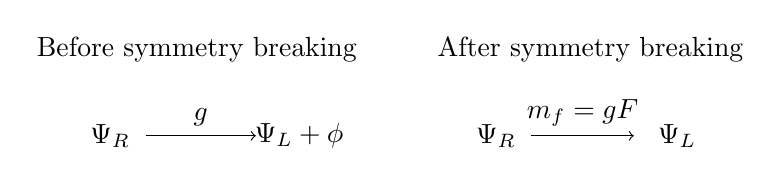
\begin{tikzpicture}[x=1cm,y=1cm]
\node at (2.0,2.1) {Before symmetry breaking};
\node at (7.0,2.1) {After symmetry breaking};
\node at (0.9,1.0) {$\Psi_R$};
\node at (3.3,1.0) {$\Psi_L+\phi$};
\draw[->] (1.35,1.0) -- (2.75,1.0) node[midway,above] {$g$};
\node at (5.8,1.0) {$\Psi_R$};
\node at (8.1,1.0) {$\Psi_L$};
\draw[->] (6.25,1.0) -- (7.55,1.0) node[midway,above] {$m_f=gF$};
\end{tikzpicture}
\caption{The Yukawa mechanism in schematic form. Before symmetry breaking, left-right conversion is accompanied by the charged scalar; after \(\phi\) is replaced by its vacuum value, the same coupling becomes an effective fermion mass.}
\end{figure}

Only in the next step, when the Higgs field takes its broken-symmetry value, does this interaction collapse into an ordinary mass term.

\section{Yukawa Masses, Neutrinos, and the Final Unification Around \(F\)}

This is where the lecture loops back to the Higgs field. Suppose the charged scalar \(\phi\) in the Yukawa term is precisely the Higgs field, and suppose it is sitting in the broken vacuum with nonzero magnitude \(F\). The phase \(\alpha\) has already been eaten by the gauge field in the gauge-boson story, so in first approximation the Higgs field contributes only its vacuum magnitude. Then
\begin{equation}
g\phi \approx gF,
\qquad
g\phi^* \approx gF,
\end{equation}
and the symmetry-allowed interaction has become an effective fermion mass:
\begin{equation}
m_f=gF.
\end{equation}
This is the fermionic analog of the gauge-boson mechanism. There the shifted Higgs background produced a term proportional to \(F^2A_\mu A^\mu\); here the same shift produces the left-right mixing coefficient \(m_f\).

But Susskind is careful not to freeze the Higgs field too completely. The Higgs is not really a rigid constant. It can fluctuate about its vacuum value, and those fluctuations are the physical Higgs boson. So schematically we should write
\begin{equation}
\phi \approx F+h,
\end{equation}
which means the Yukawa term becomes
\begin{equation}
g\phi \approx gF+gh.
\end{equation}
The first term is the fermion mass. The second is the coupling of the physical Higgs particle to that fermion. This is why the lecture treats Higgs production and decay as a future test of the whole framework: the same constant that sets the fermion mass must also control Higgs emission and Higgs decay into that fermion species.

The mass hierarchy is therefore pushed into a hierarchy of Yukawa couplings. Using the weak-boson mass scale in the loose way the lecture does, one finds for the electron
\begin{equation}
g_e \sim \frac{0.5\,\mathrm{MeV}}{10^2\,\mathrm{GeV}} \sim 10^{-5},
\end{equation}
while for the top quark the coupling is of order one,
\begin{equation}
g_t=\mathcal{O}(1).
\end{equation}
Nobody in the lecture pretends to understand that spectrum. The theory organizes the numbers, but it does not explain why the numbers are what they are. Later in the lecture Susskind quotes the symmetry-breaking scale itself as being of order \(250\,\mathrm{GeV}\); the estimate above is only an order-of-magnitude use of the observed weak-boson scale as the immediate empirical proxy for \(F\).

The neutrino discussion is lighter mathematically but conceptually important. In the simple Standard Model story, neutrinos are purely left-handed and were once thought to be massless. The lecture already treats that as only approximately true, because neutrino oscillations show that their masses are tiny but nonzero. The same basic principle still holds: for fermions, mass is left-right mixing. For a neutrino, however, the right-handed state it can mix with may be the right-handed antineutrino:
\begin{equation}
\nu_L \longleftrightarrow \bar{\nu}_R.
\end{equation}
That possibility is unavailable to the electron, because an electron cannot mix with a positron without violating charge conservation. For the neutrino there is no such electric-charge obstruction, and this is what leads Susskind to the Majorana idea: a particle whose mass arises by mixing with its own antiparticle.

The lecture closes with a broader synthesis and a caution. In the simplified presentation, all the known Standard Model masses trace back to the same symmetry-breaking scale \(F\). Gauge bosons are massless before symmetry breaking because gauge symmetry forbids a bare mass. Fermions are massless before symmetry breaking because weak interactions distinguish left from right, so the direct left-right mass term is also forbidden. After the Higgs field shifts away from the symmetric vacuum, both obstacles are bypassed.

But the lecture also stresses that not every conceivable particle need be of this protected type. If some heavy particle had left-handed and right-handed components carrying the same weak charges, there would be no symmetry obstruction to an arbitrarily large bare mass unrelated to \(F\). Such particles, if they exist, would naturally live at scales much larger than the electroweak one and would simply not yet have been seen. In that sense the familiar particle spectrum may be biased: what we have observed most clearly are precisely those particles whose masses had to wait for the Higgs field to shift.

\section{Summary}

The lecture unfolds in two parallel stories. First, the Higgs mechanism is rebuilt for gauge bosons in the simplest possible \(U(1)\) setting. A derivative-only gauge Lagrangian gives no energy for a homogeneous field shift and therefore describes a massless gauge boson. Once the Higgs field is frozen at nonzero radius and its phase is absorbed into the gauge potential, a no-derivative \(A_\mu A^\mu\)-type term appears, and the gauge boson becomes massive.

Second, the same logic is repeated for fermions. The mass term in the Dirac equation is identified with left-right mixing. But weak interactions distinguish left from right so sharply that a bare mass term is forbidden. The Yukawa coupling to the Higgs field is the symmetry-respecting way out, and once the Higgs field takes its vacuum value, that coupling becomes \(m_f=gF\). The later neutrino discussion extends the same idea toward Majorana mass.

That is the central unification of the lecture. In this simplified companion-note version, the gauge-boson masses and the fermion masses are not separate miracles. They are different responses to the same fact: the Higgs field does not sit at the symmetric point. Without that shift, the familiar particles of the Standard Model would remain massless.